\documentclass[12pt,a4paper]{report}

% --- Font and Language Settings ---
\usepackage[utf8]{inputenc}
\usepackage[T1]{fontenc}
\usepackage{newtxtext,newtxmath} % Times New Roman equivalent
\usepackage{graphicx}
\usepackage{hyperref}
\usepackage[explicit]{titlesec}
\usepackage{indentfirst}
\usepackage{setspace}
\usepackage{chngcntr}
\counterwithout{figure}{chapter}
\counterwithout{table}{chapter}
\usepackage{float}
\usepackage{booktabs}
\usepackage{multirow}
\usepackage{array} 
\usepackage{enumitem} % Required for the [nosep] and [leftmargin] options
% --- Titles Formatting (14 to 16 points) ---

% Chapter titles: Only number and title (16pt), e.g., "1. Introduction"
\titleformat{\chapter}
  {\normalfont\fontsize{16}{19}\bfseries}
  {\thechapter. }
  {0pt}
  {#1}
\titlespacing*{\chapter}{0pt}{-20pt}{20pt}

% Section titles (15pt)
\titleformat{\section}
  {\normalfont\fontsize{15}{18}\bfseries}{\thesection}{1em}{#1}

% Subsection titles (14pt)
\titleformat{\subsection}
  {\normalfont\fontsize{14}{17}\bfseries}{\thesubsection}{1em}{#1}

\begin{document}

% --- Front Page ---
\begin{titlepage}
    \centering
    \vspace*{1cm}
    {\fontsize{20}{24}\selectfont \textbf{My Coach}} \\
    \vspace{1.5cm}
    {\large Mohamed Ali Knis \\ Student Name 2 \\ Student Name 3 \\ Student Name 4 \\} 
    \vspace{1cm}
    {\large Academic Year 2025-2026} \\
    \vfill
    {\large Institution: \textbf{[\Large Higher Institute of Computer Science and Mathematics of Monastir]}} \\
    \vspace*{0.5cm}
    {\large Instructor: \textbf{[Mme. Laataoui Senda]}} \\
    \vspace{0.8cm}
    \vspace{0.8cm}
    {\large \today}
\end{titlepage}
\setstretch{1.25}
% --- Table of Contents ---
\pagenumbering{roman} 
\tableofcontents
\newpage
\listoffigures
\newpage
\listoftables
\newpage
\newpage

\pagenumbering{arabic} 
\setcounter{page}{1}  

% --- 1. Introduction ---
\chapter{Introduction and Presentation of the Idea}

\section{Context and Objectives}
In recent years, the demand for personalized fitness and nutrition solutions has surged, driven by a growing awareness of health and wellness. However, many individuals struggle to find a \textbf{single, accessible platform} that combines training programs, nutritional guidance, and community support. This project aims to address this gap by developing \textbf{``My Coach''}, a web application designed to \textbf{simplify fitness management} and provide users with a \textbf{comprehensive, interactive experience}.

The primary objective of ``My Coach'' is to offer a \textbf{user-friendly platform} where individuals can access personalized training programs, track their progress, and engage with a community of like-minded users. By integrating these features, the application seeks to \textbf{motivate users, enhance their fitness journey, and promote long-term health habits}.

\section{The Original Idea}
\textbf{``My Coach''} is a \textbf{web-based fitness platform} that provides users with tailored training programs, nutrition plans, and a supportive community. The application allows users to:
\begin{itemize}
    \item Select and follow \textbf{personalized workout programs} based on their fitness goals and experience level.
    \item Access \textbf{customized nutrition plans} to complement their training.
    \item Engage with a \textbf{community} through challenges, leaderboards, and shared achievements.
    \item Purchase \textbf{fitness products and supplements} directly from the platform.
\end{itemize}

The platform is designed with a \textbf{clean, intuitive interface} to ensure ease of use, making it accessible to both beginners and experienced fitness enthusiasts.

\section{Defense of the Idea}
The development of ``My Coach'' is justified by several key factors:
\begin{itemize}
    \item \textbf{Simplicity}: The platform consolidates multiple fitness tools into a \textbf{single, easy-to-use application}, eliminating the need for users to juggle multiple apps or services.
    \item \textbf{Personalization}: By offering tailored programs and nutrition plans, ``My Coach'' ensures that users receive \textbf{relevant, effective guidance} based on their individual needs.
    \item \textbf{Community Engagement}: The inclusion of a community feature fosters \textbf{motivation and accountability}, which are critical for long-term fitness success.
    \item \textbf{Educational Value}: The platform educates users about fitness and nutrition, empowering them to make \textbf{informed decisions} about their health.
\end{itemize}

In summary, ``My Coach'' is more than just a fitness app—it’s a \textbf{complete platform} that helps users reach their health and fitness goals.

% --- 2. Design ---
\chapter{Conception and Design}
\section{Introduction}
At this point, we're reaching a milestone in the project elaboration process. In order to have a global and highlight the major outlines, we need to transform these requirements into diagrams using UML. These charts summarize the actions that our users can perform while using our application.
\section{Main Use Case Diagram}
The figure below shows the general use case diagram of our application. This illustration will help to have a global view on the board outlines of our system and the main actions are summarized into use cases. We find as agreed the main actors and their interactions with the service.
\vspace{0.8cm}

\begin{table}[H]
    \centering
    \renewcommand{\arraystretch}{2.3} 
    \caption{Details of the main use case diagram}
    \vspace{0.4em}
        \begin{tabular}{|p{3.5cm}|p{8.5cm}|}
        \hline
        \textbf{Title :} & 
        \begin{itemize}[label=$\bullet$, leftmargin=*, nosep, before=\vspace{-0.6\baselineskip}]
            \item Main Use Case Diagram
        \end{itemize} \\ \hline
        
        \textbf{Actors :} & 
        \begin{itemize}[label=$\bullet$, leftmargin=*, nosep, before=\vspace{-0.6\baselineskip}]
            \item User
        \end{itemize} \\ \hline
        
        \textbf{Precondition :} & 
        \begin{itemize}[label=$\bullet$, leftmargin=*, nosep, before=\vspace{-0.6\baselineskip}]
            \item Internet connection required
        \end{itemize} \\ \hline
        
        \textbf{Description :} & 
        \begin{itemize}[label=$\bullet$, leftmargin=*, nosep, before=\vspace{-0.6\baselineskip}]
            \item The user can use the website to access various information regarding physical training
            \item The system running in the background will import the data and trigger in specific cases.
        \end{itemize} \\ \hline
        
        \textbf{Post conditions :} & 
        \begin{itemize}[label=$\bullet$, leftmargin=*, nosep, before=\vspace{-0.6\baselineskip}]
            \item Displayed interfaces
        \end{itemize} \\ \hline
    \end{tabular}
\end{table}
\begin{figure}[H]
    \vspace{-3cm}
    \hspace{-3cm}
    \centering   
    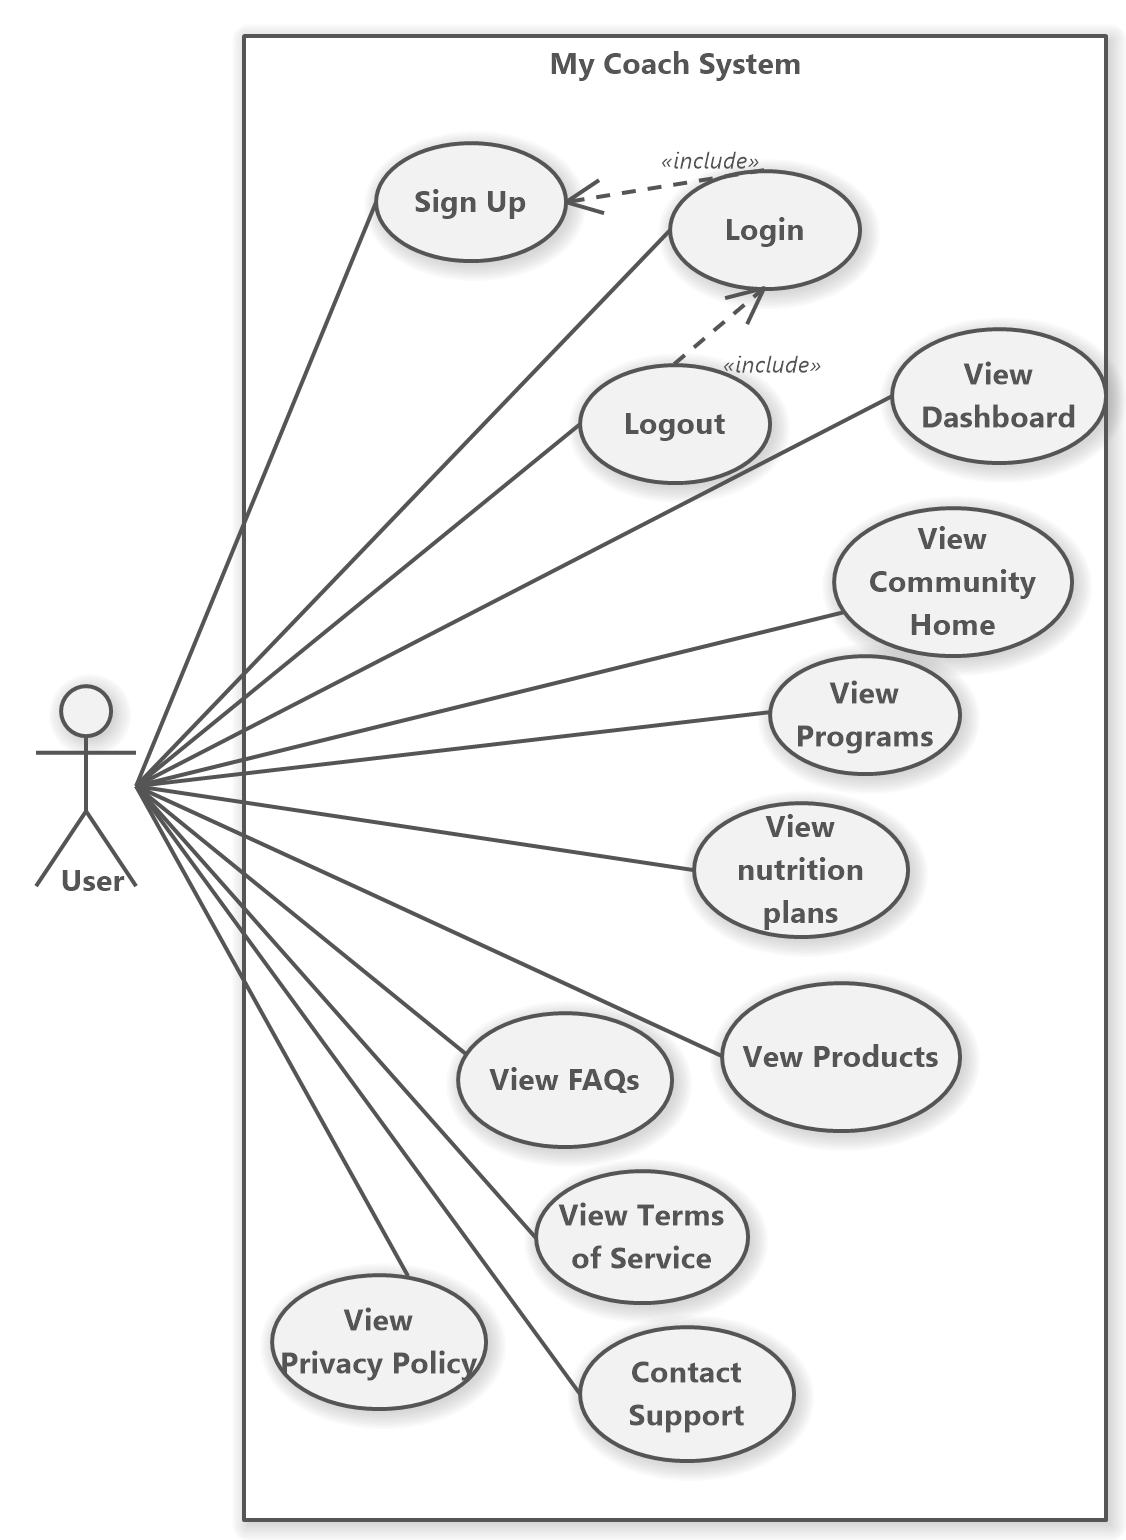
\includegraphics[width=1.2\textwidth]{General_uc1.png}
    \vspace{0.1em}
    \caption{General Use Case}
    \label{fig:general_use_case}
\end{figure}
\section{Detailed Use Cases}
In this part of this chapter, we are going to give a closer look at the different use cases mentioned in the previous diagram. This will give us a more defined idea of the flow process for a given functionality that the user can execute.
\subsection{Use case diagram for view programs}
The tables below sum up the use case "View Programs" It describes the actor and the conditions of our process.
\begin{table}[H]
    \centering
    \renewcommand{\arraystretch}{2.3} 
    \caption{Details of View Programs use case diagram}
    \vspace{0.4em}
        \begin{tabular}{|p{3.5cm}|p{8.5cm}|}
        \hline
        \textbf{Title :} & 
        \begin{itemize}[label=$\bullet$, leftmargin=*, nosep, before=\vspace{-0.6\baselineskip}]
            \item View Programs use case diagram
        \end{itemize} \\ \hline
        
        \textbf{Actors :} & 
        \begin{itemize}[label=$\bullet$, leftmargin=*, nosep, before=\vspace{-0.6\baselineskip}]
            \item User
            \item The System
        \end{itemize} \\ \hline
        
        \textbf{Precondition :} & 
        \begin{itemize}[label=$\bullet$, leftmargin=*, nosep, before=\vspace{-0.6\baselineskip}]
            \item Internet connection required
            \item Authentication required
        \end{itemize} \\ \hline
        
        \textbf{Description :} & 
        \begin{itemize}[label=$\bullet$, leftmargin=*, nosep, before=\vspace{-0.6\baselineskip}]
            \item The user will fill a form in which he will select his body biometrics.
            \item Based on this information, the system will show recommended programs.
            \item Among these programs, the user will select one of them.
        \end{itemize} \\ \hline
        
        \textbf{Post conditions :} & 
        \begin{itemize}[label=$\bullet$, leftmargin=*, nosep, before=\vspace{-0.6\baselineskip}]
            \item Selected program
        \end{itemize} \\ \hline
    \end{tabular}
\end{table}
\begin{figure}[H]
    \vspace{-3cm}
    \hspace{-2.5cm}
    \centering   
    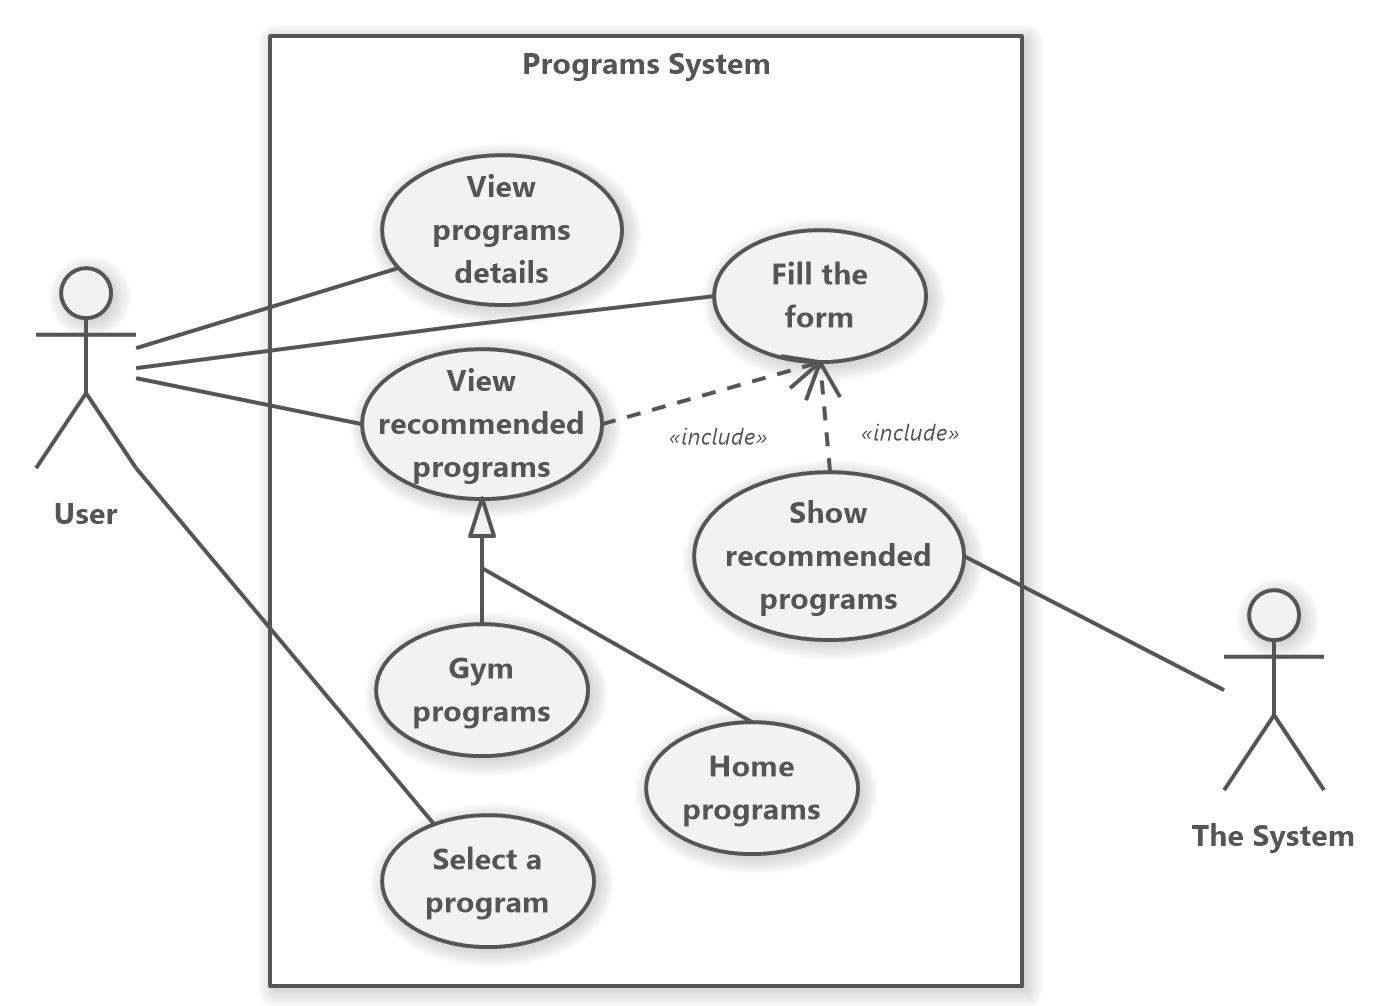
\includegraphics[width=1.2\textwidth]{Programs_uc2.png}

    \caption{View Programs use case diagram}
    \label{fig:programs_use_case}
\end{figure}
\subsection{Use case diagram for View community home}
The tables below sum up the use case "View Community home" It describes the actor and the conditions of our process.
\begin{table}[H]
    \centering
    \renewcommand{\arraystretch}{1} 
        \caption{Details of View Community home use case diagram}
    \vspace{0.4em}
        \begin{tabular}{|p{3.5cm}|p{8.5cm}|}
        \hline
        \textbf{Title :} & 
        \begin{itemize}[label=$\bullet$, leftmargin=*, nosep, before=\vspace{-0.6\baselineskip}]
            \item View Community Home use case diagram
        \end{itemize} \\ \hline
        
        \textbf{Actors :} & 
        \begin{itemize}[label=$\bullet$, leftmargin=*, nosep, before=\vspace{-0.6\baselineskip}]
            \item User
        \end{itemize} \\ \hline
        
        \textbf{Precondition :} & 
        \begin{itemize}[label=$\bullet$, leftmargin=*, nosep, before=\vspace{-0.6\baselineskip}]
            \item Internet connection required
            \item Authentication required
        \end{itemize} \\ \hline
        
        \textbf{Description :} & 
        \begin{itemize}[label=$\bullet$, leftmargin=*, nosep, before=\vspace{-0.6\baselineskip}]
            \item The user can browse the leaderboard, achievements, and stats
            \item The user can join a challenge and earn points if it's completed. 
        \end{itemize} \\ \hline
        
        \textbf{Post conditions :} & 
        \begin{itemize}[label=$\bullet$, leftmargin=*, nosep, before=\vspace{-0.6\baselineskip}]
            \item Community leaderboard, recent achievements and stats interfaces displayed
        \end{itemize} \\ \hline
    \end{tabular}
\end{table}
\begin{figure}[H]
    \vspace{-3cm}
    \hspace{-3cm}
    \centering   
    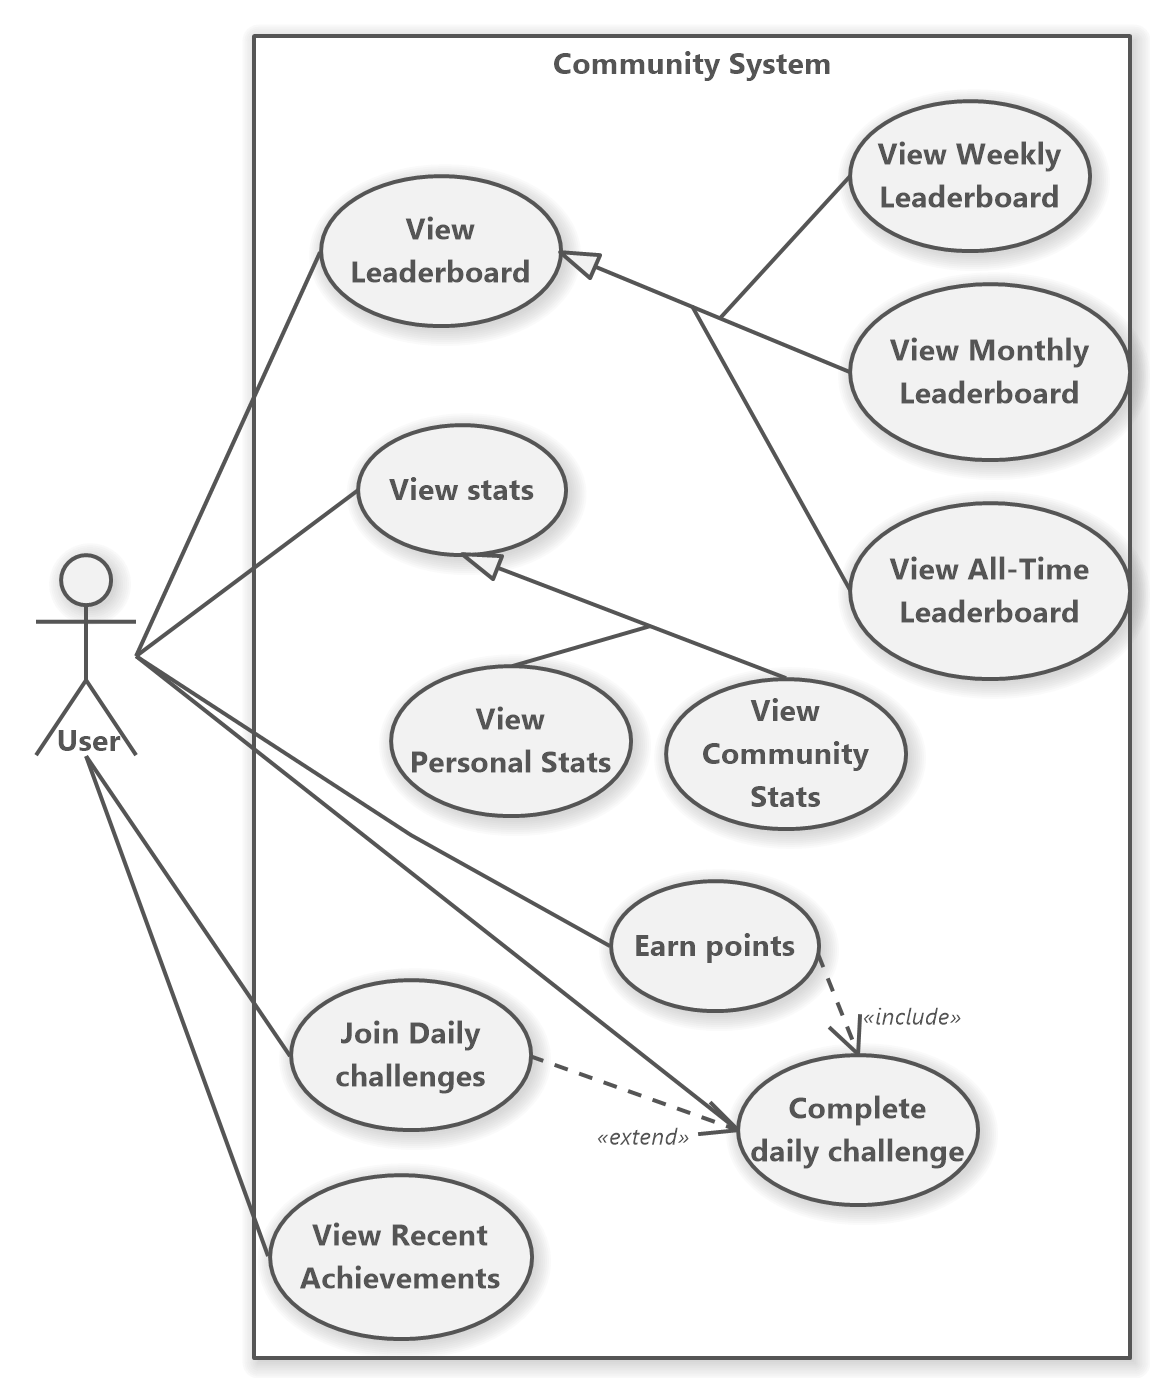
\includegraphics[width=0.75\textwidth]{Community_uc.png}
    \caption{View Community use case diagram}
    \label{fig:community_use_case}
\end{figure}
\subsection{Use case diagram for View Products}
The tables below sum up the use case "View Products" It describes the actor and the conditions of our process.
\begin{table}[H]
    \centering
    \renewcommand{\arraystretch}{1} 
        \caption{Details of View Products use case diagram}
    \vspace{0.4em}
        \begin{tabular}{|p{3.5cm}|p{8.5cm}|}
        \hline
        \textbf{Title :} & 
        \begin{itemize}[label=$\bullet$, leftmargin=*, nosep, before=\vspace{-0.6\baselineskip}]
            \item View Products use case diagram
        \end{itemize} \\ \hline
        
        \textbf{Actors :} & 
        \begin{itemize}[label=$\bullet$, leftmargin=*, nosep, before=\vspace{-0.6\baselineskip}]
            \item User
            \item Payment Gateway
        \end{itemize} \\ \hline
        
        \textbf{Precondition :} & 
        \begin{itemize}[label=$\bullet$, leftmargin=*, nosep, before=\vspace{-0.6\baselineskip}]
            \item Internet connection required
            \item Authentication required
            \item Have a payment card
        \end{itemize} \\ \hline
        
        \textbf{Description :} & 
        \begin{itemize}[label=$\bullet$, leftmargin=*, nosep, before=\vspace{-0.6\baselineskip}]
            \item The user can buy sporting equipment and supplements.
        \end{itemize} \\ \hline
        
        \textbf{Post conditions :} & 
        \begin{itemize}[label=$\bullet$, leftmargin=*, nosep, before=\vspace{-0.6\baselineskip}]
            \item Product Purchased
        \end{itemize} \\ \hline
    \end{tabular}
\end{table}
\begin{figure}[H]
    \vspace{-3cm}
    \hspace{-3cm}
    \centering   
    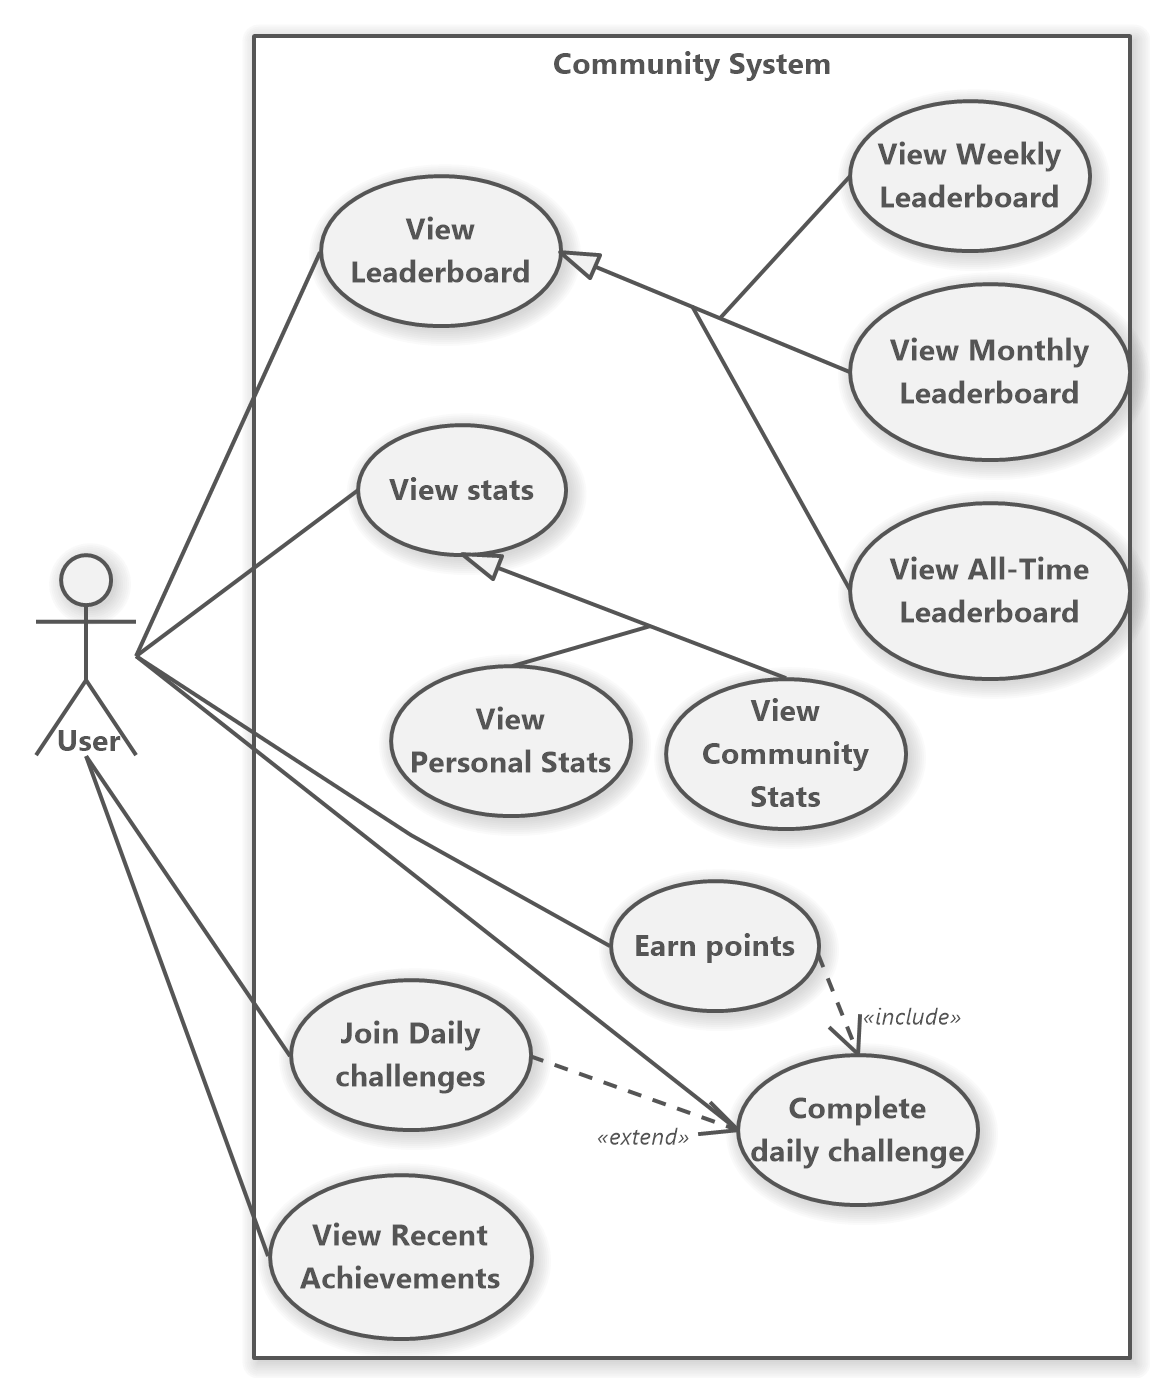
\includegraphics[width=1.2\textwidth]{Community_uc.png}
    \caption{View Products use case diagram}
    \label{fig:products_use_case}
\end{figure}
\section{Sequence Diagrams}

\subsection{Authentication}
\begin{figure}[H]
    \centering
    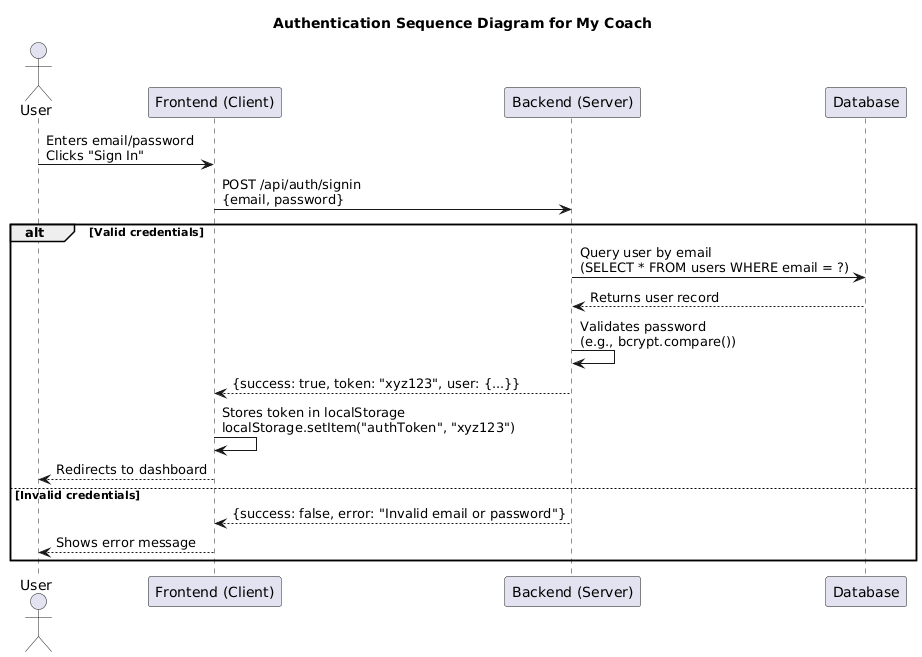
\includegraphics[width=0.9\textwidth]{Authentication_Sequence.png}
    \caption{Sequence diagram for user authentication in "My Coach".}
    \label{fig:auth_sequence}
\end{figure}

\subsection{Choosing a Training Program}
\begin{figure}[H]
    \centering
    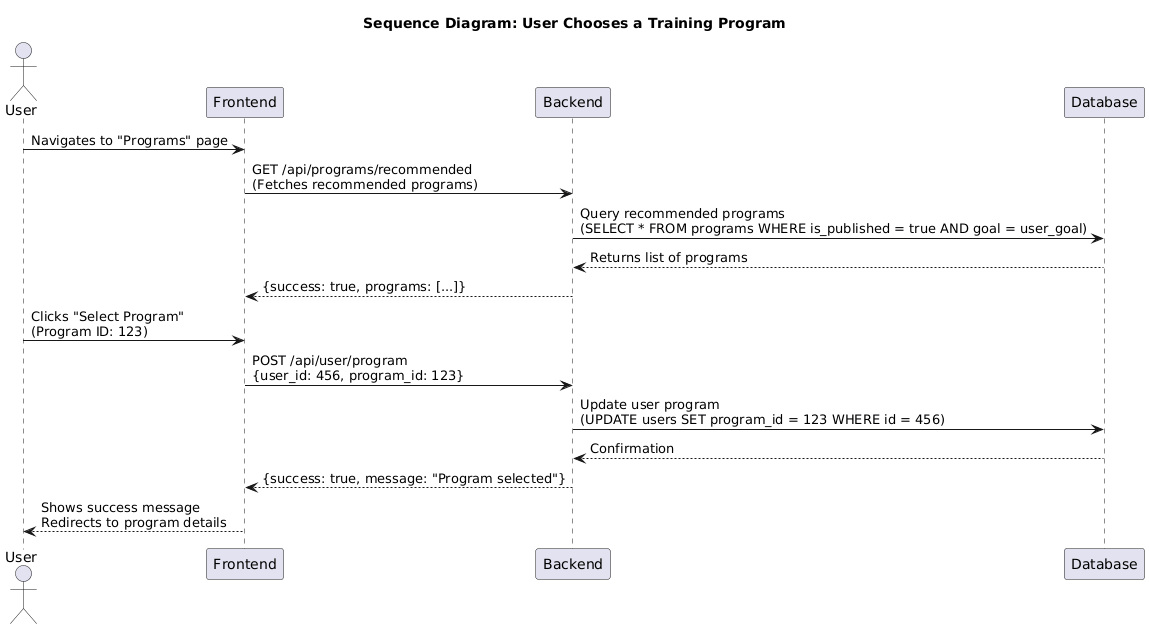
\includegraphics[width=0.9\textwidth]{Choose_Program_Sequence.png}
    \caption{Sequence diagram for choosing a training program.}
    \label{fig:choose_program}
\end{figure}

\subsection{Choosing a Nutrition Plan}
\begin{figure}[H]
    \centering
    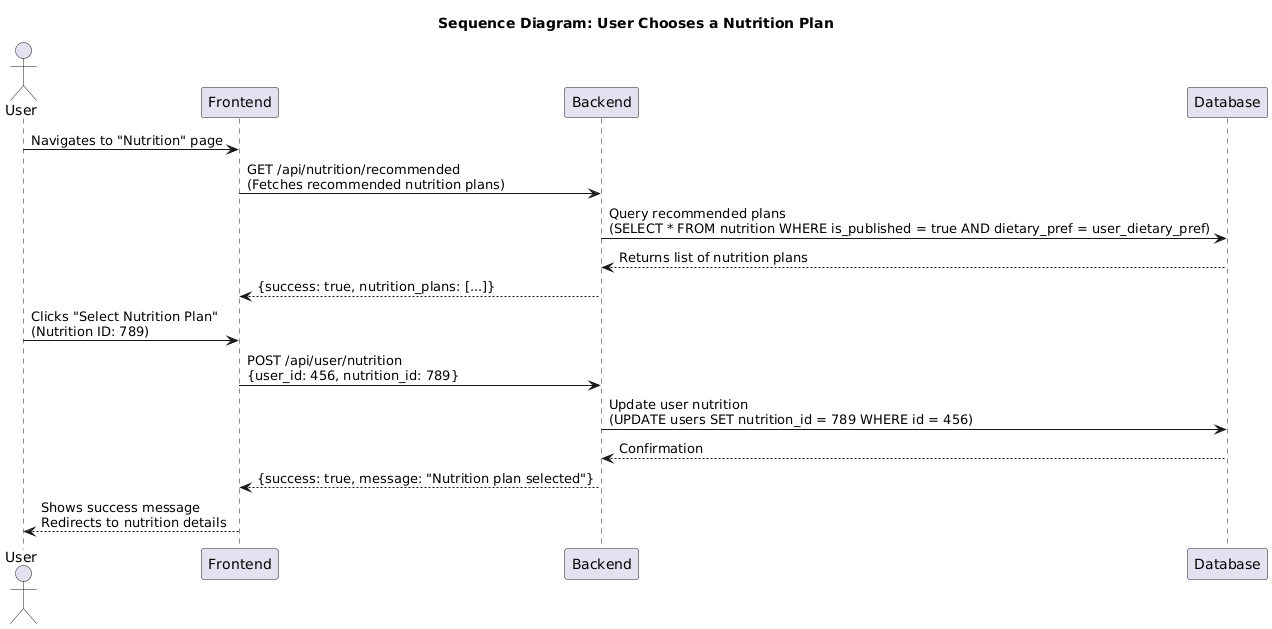
\includegraphics[width=0.9\textwidth]{Choose_Nutrition_Sequence.png}
    \caption{Sequence diagram for choosing a nutrition plan.}
    \label{fig:choose_nutrition}
\end{figure}

\subsection{Filling the User Profile Form}
\begin{figure}[H]
    \centering
    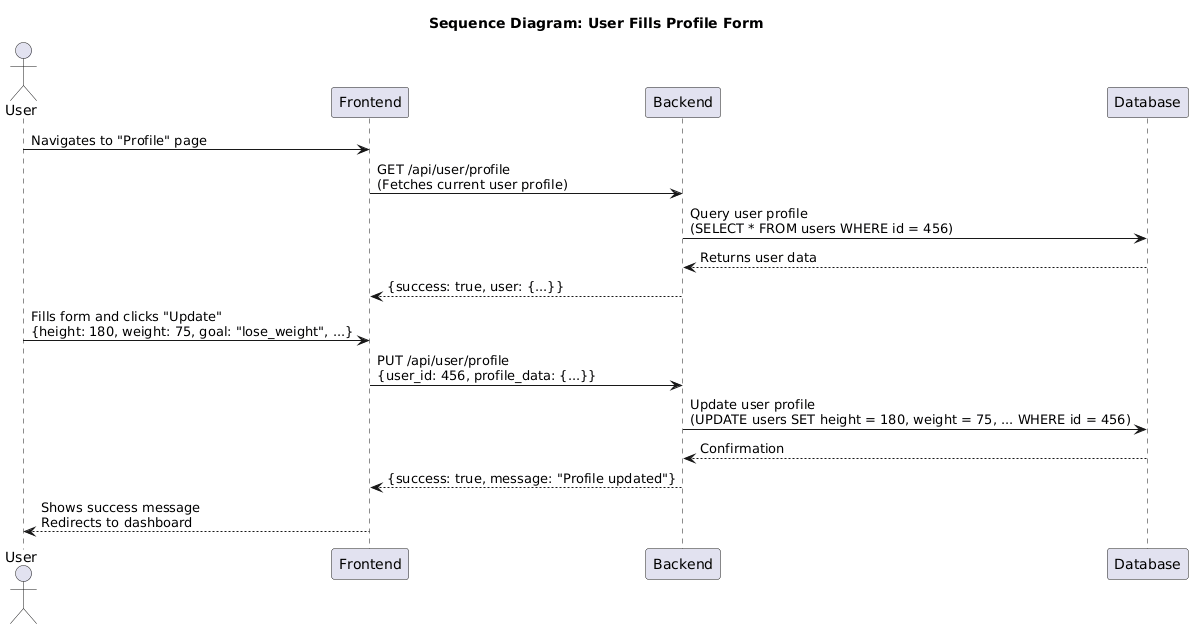
\includegraphics[width=0.9\textwidth]{Fill_Profile_Sequence.png}
    \caption{Sequence diagram for filling the user profile form.}
    \label{fig:fill_profile}
\end{figure}

\section{Additional Diagrams}
\section{Technical Architecture (Mobile/Backend/Database)}
The technical architecture is structured into four parts: the client, web server, application server, and database. On the client side we  use HTML, CSS, and JavaScript, which run on the user’s browser and are responsible for displaying the interface and sending HTTP/HTTPS requests according to user actions. The web server (e.g. Nginx) handles the requests and passes API calls to the backend. The application server is based on the Backend-as-a-Service Supabase, which implements the business logic executing methods and triggers written in PL/SQL in the SQL editor and exposes RESTful APIs automatically. The database layer, based on PostgreSQL, takes care of data storage, management, and integrity and, when needed, the execution of triggers and procedures. Data flows from the client to the web server, then to Supabase and the database, before returning the processed results back to the user.

\begin{figure}[H]
    \centering
    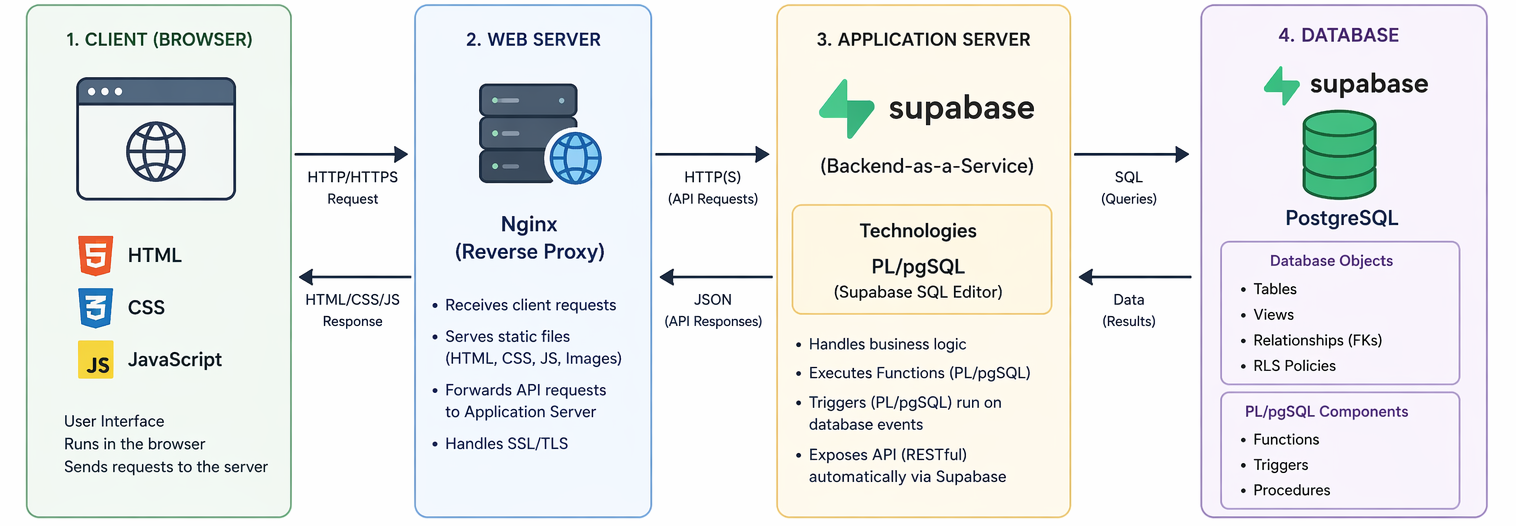
\includegraphics[width=1\linewidth]{arch.png}
    \caption{Architecure schema}
    \label{fig:placeholder}
\end{figure}
\section{Mockups }
\subsection{Main page}
Landing Page It’s the main entry point. There’s a value proposition in the center and a simple “Hero” section. The ergonomic layout works well, creating a powerful focal point that immediately conveys the platform's objective. We simplified the navigation bar to only include necessary features to reduce “choice overload.” We also positioned the profile symbol in the upper-right corner to match universal user mental models for easy account access..
\begin{figure}[H]
    \centering
    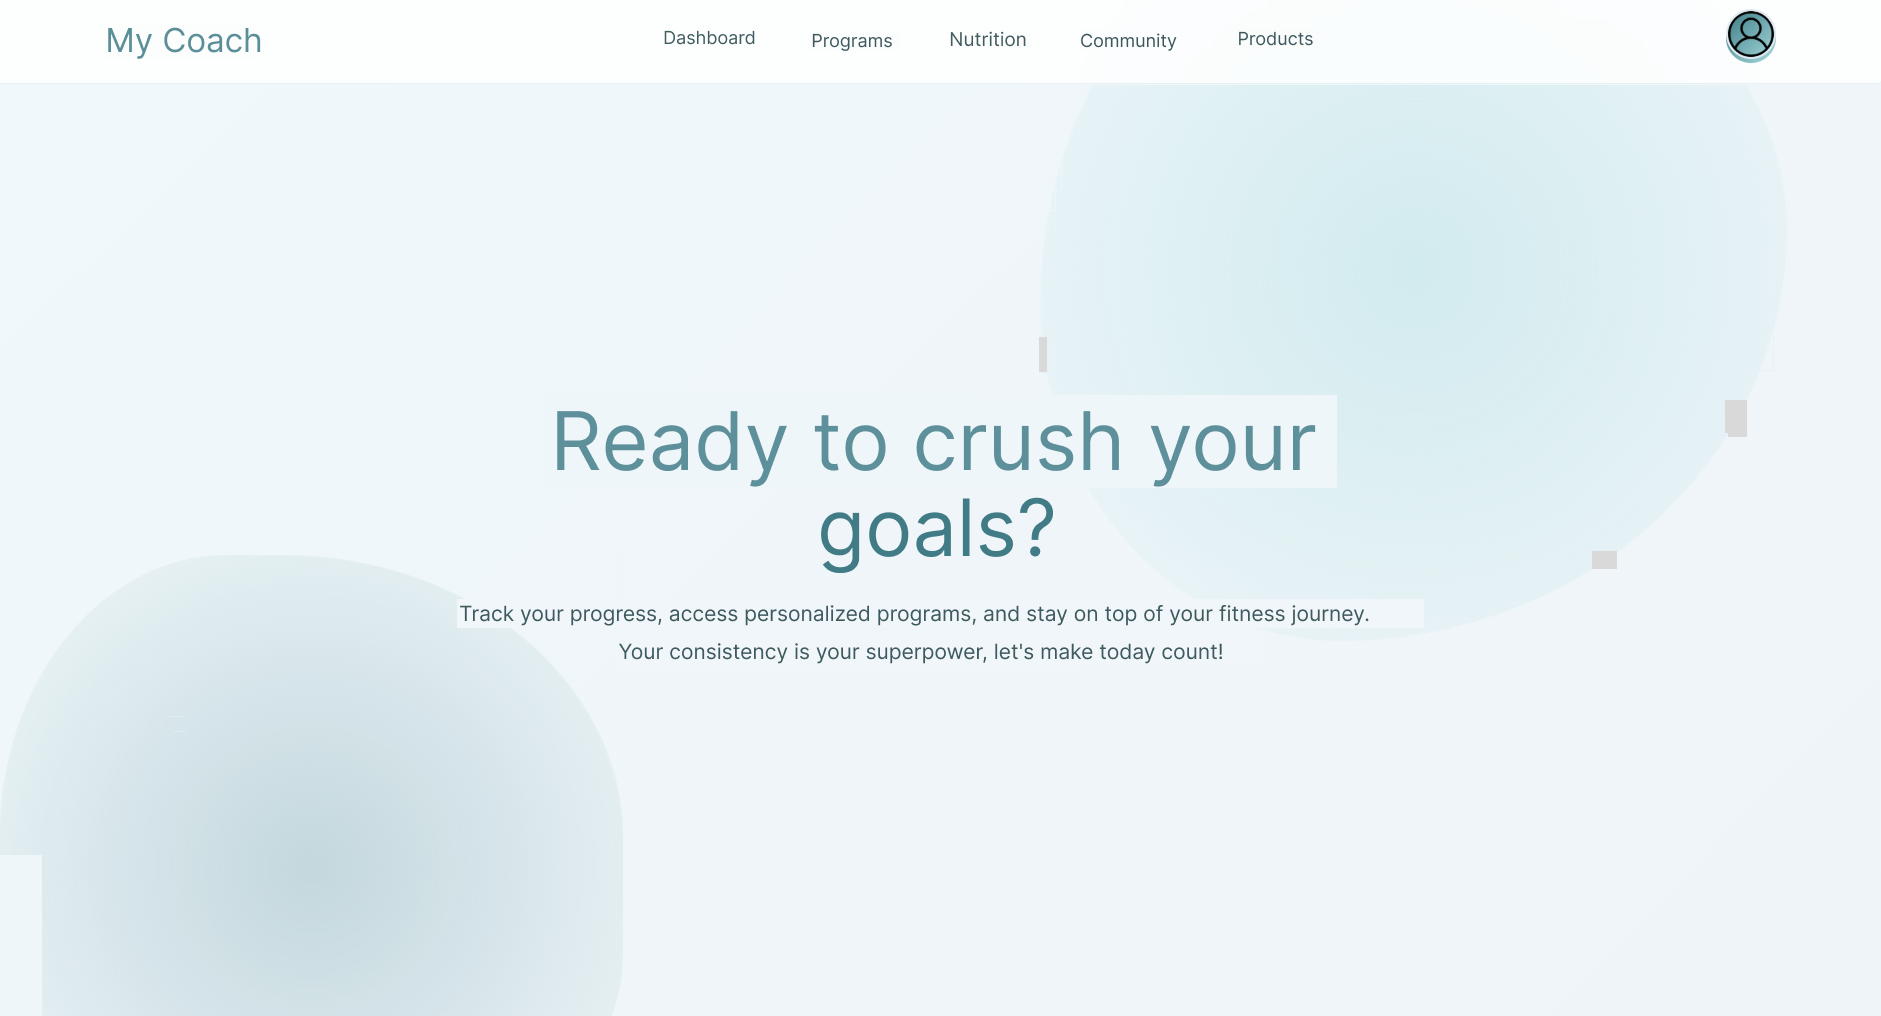
\includegraphics[width=0.85\linewidth]{main_page.png}
    \caption{Main page Mockup}
    \label{fig:placeholder}
\end{figure}
\subsection{Features page}
The “What We Offer” section showcases the main services provided by the platform in a card-based modular layout. The technique utilizes “Information Chunking”, which helps users quickly grasp a wide variety of products, including personalized programs and nutrition, without feeling cognitively exhausted. The great use of white space and consistent card padding, which makes the interface look professional and offers great readability, makes the interface feel open and friendly to novice users.
\begin{figure}[H]
    \centering
    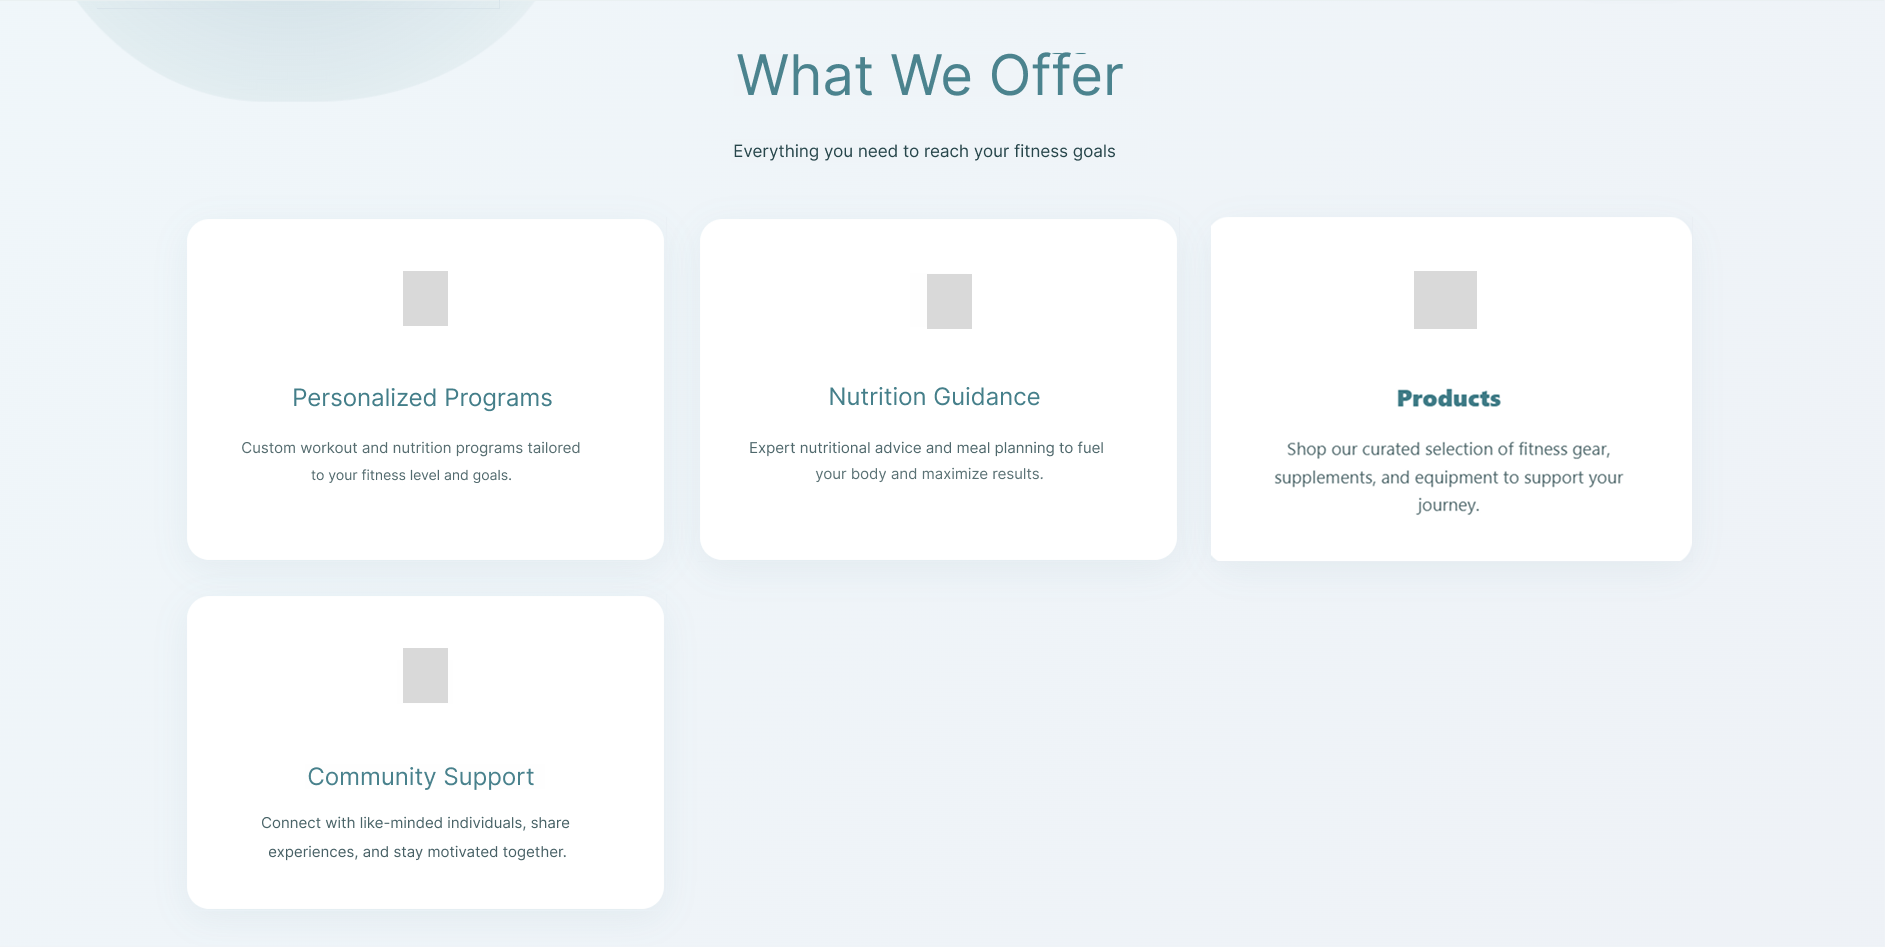
\includegraphics[width=0.85\linewidth]{features_before_login.png}
    \caption{Features page Mockup}
    \label{fig:placeholder}
\end{figure}
\subsection{Sign Up page}
The input fields on the Sign-up screen are in a logical order from basic identity (Username/Email) to security credentials. The linear flow reduces onboarding friction by aligning with user expectations. That same “Sign in” link at the bottom is also an important “navigation anchor” that makes it easy for visitors to change context if they already have an account. This improves the flow of the user journey.
\begin{figure}[H]
    \centering
    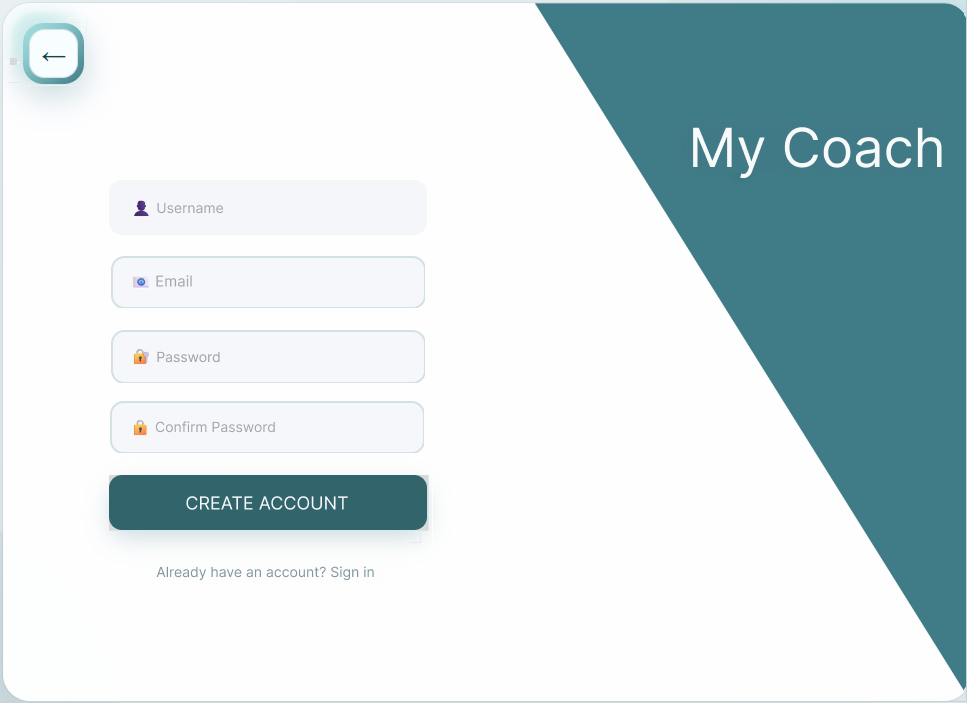
\includegraphics[width=0.75\linewidth]{signup.png}
    \caption{Sign Up page Mockup}
    \label{fig:placeholder}
\end{figure}

% --- 3. Development ---
\chapter{Development}
\section{Chosen Technologies and Justifications}
\section{Code Organization}
\section{Implementation of Key Features}
\section{Data Management}

% --- 4. Testing and Validation ---
\chapter{Testing and Validation}
\section{Test Environment and Tools}
\section{Test Scenarios}

% --- 5. Conclusion and Perspectives ---
\chapter{Conclusion and Perspectives}
\section{Project Assessment}
\section{Global Difficulties and Learnings}
\section{Possible Evolutions}

% --- 6. Appendices ---
\chapter{Appendices}
\section{Link to Git Repository}
\section{Supplementary Screenshots}
\section{Configuration Files}

\end{document}
